
%
%  $Description: Author guidelines and sample document in LaTeX 2.09$ 
%
%  $Author: ienne $
%  $Date: 1995/09/15 15:20:59 $
%  $Revision: 1.4 $
%

\documentclass[times, 10pt,twocolumn]{article} 
\usepackage{latex8}
\usepackage{times}
\usepackage[utf8]{inputenc}
\usepackage[brazil]{babel}
\usepackage{graphicx, url}
\usepackage{listings}
\usepackage[num]{abntex2cite}
\usepackage[center]{caption}

\usepackage[usenames]{color}

\definecolor{red}{rgb}{0.6,0,0} % for strings
\definecolor{green}{rgb}{0.25,0.5,0.35} % comments
\definecolor{purple}{rgb}{0.5,0,0.35} % keywords
\definecolor{docblue}{rgb}{0.25,0.35,0.75} % javadoc

\definecolor{DarkBlue}{rgb}{0,0,0.61}
\definecolor{DarkGreen}{rgb}{0,0.4,0}

\lstset{
  language=vhdl,
  basicstyle=\ttfamily\fontsize{10}{11}\selectfont,
  keywordstyle=\color{purple}\bfseries,
  stringstyle=\color{red},
  commentstyle=\color{green},
  morecomment=[s][\color{docblue}]{/*}{*/},
  numbers=left,
  numberstyle=\tiny\color{black},
  stepnumber=1,
  numbersep=10pt,
  tabsize=4,
  showspaces=false,
  showstringspaces=false,
  otherkeywords={\#include, \#define, \#pragma, \#typedef, dim3},
  emph={ __device__, __global__, __shared__, __host__, __constant__},
  emphstyle=\color{DarkBlue}\bfseries,
  emph={[2] printf, scanf},
  emphstyle=[2]\color{DarkGreen},
  extendedchars=true,
  frame=tb,
  breaklines=true
}

\usepackage{caption}
\DeclareCaptionFont{black}{\color{black}}

\renewcommand{\lstlistingname}{Código}

\usepackage{footnote}

%------------------------------------------------------------------------- 
% take the % away on next line to produce the final camera-ready version 
\pagestyle{empty}

%------------------------------------------------------------------------- 
\begin{document}
\begin{savenotes}
\title{Título do Artigo\footnote{Trabalho desenvolvido para a disciplina de BCC34G – Sistemas Operacionais.}}


\author{Eduardo Barbosa de Oliveira, Rafael Rampin Soratto\\
Coordenação do Curso de Bacharelado em Ciência da Computação - COCIC\\
Universidade Tecnológica Federal do Paraná - UTFPR\\ 
Campus Campo Mourão\\
Campo Mourão, Paraná, Brasil\\
eduardooliveira.1997@alunos.utfpr.edu.br e segundo@email.com.br\\
% For a paper whose authors are all at the same institution, 
% omit the following lines up until the closing ``}''.
% Additional authors and addresses can be added with ``\and'', 
% just like the second author.
}

\maketitle
\thispagestyle{empty}

\begin{abstract}
    O presente relatório desmontrará e explicará a implementação e o funcionamento de um simulador de gerenciador de processos implementado em Python. Trará também, uma introdução aos quatro algoritmos de escalonamentos de processos que foram implementados, sendo eles: FIFO (First in First out), SJF (Short Job First), Prioridade e RR (Round-Robin).
\end{abstract}
%------------------------------------------------------------------------- 
\section{Introdução} \label{sec_introducao}
    Os quatro alrotimos de escalonamento implentados são: FIFO, que tem como base uma fila onde o primeiro processo á chegar é o primeiro a sair; SFJ, que executará primeiro sempre o menor processo; RR, que tem como base uma fila circular que executará pequenas partes do processo à cada iteração da fila; Prioridade, que os processos recebem um atributo de prioridade para definir quem executará primeiro.
%-------------------------------------------------------------------------
% Salva as notas de rodapé na primeira página.
\end{savenotes}

\section{Processos}
    Um processo é basicamente um programa em execução. Cada processo tem associado o seu espaço de enderaçamento, que consiste numa lista de posições, que vai de zero até um máximo, que o processo pode fazer operações de leitura e escrita. Nesse enderaçamento de memória, está disponível o programa executável, os dados do programa e sua pilha. Também está associado com um processo, um conjunto de recursos que contém registradores, uma lista de arquivos abertos, alarmes pendentes, lista de processos relacionados e todas as informações que serão necessárias para a execução do programa.\cite{tanenbaum}
\subsection{Tipos de processos}
    Existem três tipos de processo no nosso contexto: IO Bound, CPU Bound e misto.
    
    Processos IO Bound são aqueles processos que precisa esperar até que uma operação de entrada/saída(Input/Out) sejam completadas. Eles são um problema já que precisam interromper a execução para esperar o termino das operações de IO.
    
    Já os processos CPU Bound são processos que só dependem da CPU para execução, ou seja, o tempo de execução do processo é definido exclusivamente pela velocidade de processamento da CPU, sem precisar esperar eventos de IO.
    
    Os processos misto, como o nome sugere, é uma mistura de CPU Bound e IO Bound, ou seja, é um processo que contém o uso da CPU e necessita esperar eventos de IO. Esses serão os mais comuns nesse relatório.
    
%------------------------------------------------------------------------- 
\section{Gerenciador de processos} \label{sec_escalonamento}
    O gerenciador de processos é responsável por executar o escalonamento de processos de forma que respeite as estratégias particulares de cada tipo de escalonamento de processos (FIFO, Round-Robin, Prioridade e outros).\cite{tutorialspoint}Ele tem o poder de parar e voltar à executar qualquer processo.
    
    O escalonamento de processos é peça fundamental em sistemas operacionais de Multiprogramação, pois esses sistemas permitem a execução de mais de um programa de uma vez, sendo assim, precisando carregar para a memória o contexto do processo e fazendo a troca de contexto baseado em cada estratégia de escalonamento de processos.
    
    Um escalonamento de processos pode ser de dois tipos: preemptivo e cooperativo, ou não preemptivo. O preemptivo é capaz de interromper, alterar o estado de execução do processo e começar executar outro, já o cooperativo, o processo que está sendo executado não pode ser interrompido.\cite{rutgers}
    
    Existem três tipos de escalonadores de processos: curto prazo, médio prazo e longo prazo.
\subsection{Curto prazo}
    O escalonador de curto-prazo (também conhecido como Escalonador da CPU) decide qual será o proximo processo à ser executado depois da interrupção do clock, uma interrupção de IO, uma operação de chamada de sistema ou outro sinal.\cite{wiki} Ele também pode alterar o estado do processo, de pronto para executando. Quando ele faz essa troca de estado e começa a executar o processo, ele faz a alocação da CPU para o mesmo.
\subsection{Médio prazo}
    O escalonador de médio prazo é uma parte da \emph{troca}. É ele quem: remove um processo da memória, reduz o grau de multiprogramação e faz a \emph{troca} dos procesos de saída.
    
    Imaginemos a seguinte situação, um processo é suspendido para um evento de IO. Um processo que está suspenso para IO não irá fazer nenhum progresso para terminar, sendo assim, o processo é retirado da memória e movido para um armazenamento secundário, feito isso, irá liberar espaço para outros processos que podem fazer progresso. Esse processo é chamado de \emph{troca}.\cite{tutorialspoint} Este processo se faz necessário por manter o rendimento do sistema.

\subsection{Longo prazo}
    O escalonador de longo prazo (também conhecido como escalonador de admissão) decide quais processos vão ser admitos para a execução. Ele seleciona o processo na lista e carrega o contexto dele na memória.
    
    Seu principal objetivo é prover um escalonamento balanceado entre processos de IO e CPU. Ele também controla o grau de multiprogramação. Se o grau de multiprogramação é estável, então a quantidade de entrada de processos deve ser igual a quantidade de saídas de processos.\cite{tutorialspoint}
    
    
%Os tópicos do texto, devem possuir nomes significativos que tenham relação com o texto, no seu texto podem haver referências a outros trabalhos e artigos que foram consultados, estudados para a elaboração do trabalho. Referências devem ter o seguinte formato: [número], por exemplo \cite{Codishetal2000} refere-se ao primeiro trabalho apresentado na seção “Referências” e assim por diante no decorrer do texto.
%As figuras devem ser referenciadas no seu texto e apresentadas conforme o modelo. Por exemplo, a Figura~{\ref{fig:figura-001}} apresenta como é feito o uso dos bancos da cache pelas tarefas.

%\begin{figure}[!htb]
 %   \centering
 %   
\includegraphics{figuras/droopy.jpg}
 %   \caption{Legenda}
 %   \label{fig:figura-001}
%\end{figure}

\section{Escalonador de Processos} \label{sec_escalonador_proc}
O escalonador de processos é o componente do sistema operacional que é responsável por decidir se o processo atualmente em execução deve continuar em execução e, caso contrário, qual processo deve ser executado a seguir.\cite{rutgers} Existem quatro eventos que podem ocorrer onde o agendador precisa entrar e tomar essa decisão: 
\begin{enumerate}
\item O processo atual vai da execução para o estado de espera porque emite uma solicitação de I/O ou alguma solicitação do sistema operacional que não pode ser atendida imediatamente. 

\item O processo atual é finalizado.
\item Uma interrupção de tempo faz com que o planejador seja executado e decida que um processo foi executado para o intervalo de tempo designado e que é hora de movê-lo do estado de execução para o estado de pronto.
 
\item Uma operação de I/O é concluída para um processo que solicitou isso e o processo agora é movido do estado de espera para pronto. O escalonador pode então decidir antecipar o processo em execução no momento e mover esse processo recém-pronto para o estado de execução.  
\end{enumerate}
Os processos possuem diversas características que são fundamentais para o bom funcionamento dos escalonadores, são elas:  
\begin{itemize} 
\item "Tempo de Chegada": Utilizado no algoritmo FIFO\footnote{First In First Out};	
\item "Tamanho" : Utilizado no algoritmo SJF; 
\item "Prioridade" : Utilizado no algoritmo de Prioridades;  
\item "Quantum" : Utilizado no algoritmo Round Robin.
\end{itemize}
Portanto, os processos podem ser organizados pelas suas características antes de serem executados pela CPU, e para cada tipo de escalonamento é possível que exista uma situação de execução diferente pois a lista de processos prontos para serem executados também será diferente. Além de organizar os processos é necessário de um processo no final chamado de sistema, ele é útil pois quando acaba a execução de todos os processos de usuário então o processo sistema é chamado para realizar as I/O pendentes dos processos. Esse processo chamado sistema também pode ser acessado de diferentes formas, por exemplo: No algoritmo Round Robin temos uma lista de execução circular e no final de cada ciclo é necessário que o sistema realize todas I/O que existem até aquele determinado tempo de execução. \cite{tutorialspoint}
\begin{enumerate}
\item  Algoritmos não preemptivos são projetados de forma que, quando um processo entra no estado de execução, ele não pode ser precedido até completar o tempo alocado. Exemplos: (e.j FIFO e SJF).
\item Algoritmos Preemptivos: a intercalação mudará de acordo com as execuções de E/S do processo, ou seja, quando o processo realiza um evento de entrada e saída é necessário pausar sua execução e chamar o próximo processo de acordo com a lista de execução. Exemplos: (e.j Round Robin e Prioridades). 
\end{enumerate} 
 
 
\subsection{FIFO} 
First In Firts Out(Primeiro a entrar, primeiro a sair): é o algoritmo que escalona os processos de acordo com seu tempo de chegada. Espera o primeiro processo chegar e então lista os próximos processos. Ele é não preemptivo e relativamente simples pois sua implementação é baseada na fila FIFO. E tem fraco desempenho, pois o tempo médio de espera é alto.\cite{rutgers} 
\begin{figure}[!htb]
	\centering
	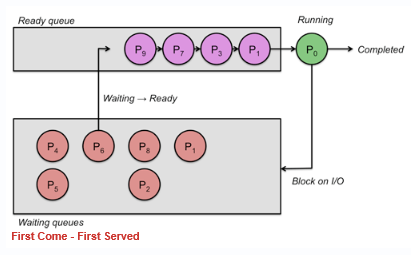
\includegraphics[width=.5\textwidth]{figuras/ilusfifo}
	\caption{Simulação FIFO} 
	\textbf{Fonte:} https://www.cs.rutgers.edu/ \cite{rutgers}
	\label{fig:figura-ilus1}
\end{figure}      
 
\subsection{SJF} 
Shorted Job First (Menor Processo Primeiro): é o algoritmo que escalona os processos de acordo com o seu tamanho. Primeiro espera o primeiro processo se ele não chegar no tempo "0" de execução, a partir dai os processos listados pelo seu tamanho de forma que sempre o menor tamanho será executado primeiro. A fila de trabalhos é classificada pelo comprimento estimado do trabalho para que os programas curtos sejam executados primeiro e não sejam retidos pelos longos, e isso minimiza o tempo médio de resposta. Como esse algoritmo não é preemptivo ele só executa as I/O dos processos depois que todos forem executados ou quando um processo terminou sua execução porém o próximo "menor processo" a ser executado ainda não chegou no seu tempo de execução. Melhor abordagem para minimizar o tempo de espera e é fácil de implementar em sistemas de lote onde o tempo de CPU necessário é conhecido antecipadamente.
Impossível implementar em sistemas interativos onde o tempo de CPU necessário não é conhecido. O processador deve saber com antecedência quanto tempo o processo levará. \cite{tutorialspoint}
Como o tempo de resposta é baseado no tempo de espera e no tempo de processamento, processos mais longos são significativamente afetados por isso. O tempo geral de espera dos processos é menor que o "FIFO", no entanto, nenhum processo precisa aguardar o término do processo mais longo.
A fome é possível, especialmente em um sistema ocupado com muitos processos pequenos sendo executados, logo os processos de maior tamanho tem dificuldade ou demoram para ter acesso a CPU, o que chama-se de fome. \cite{rutgers}

\subsection{Round Robin} 
Esse algoritmo escalona os processos de acordo com seu tempo de chegada, porém ele possui um "quantum" de execução que gera uma lista circular: Primeiro é executado um quantum de cada processo, se o tamanho do processo for menor que esse quantum então ele pode ser executado por completo, depois de cada rodada de execução do quantum o processo sistema é chamado para realizar as entradas e saídas e esse processo se repete até que todos processos terminem sua execução e I/O. Ele é considerado um algoritmo preemptivo pois sua fila circular de execução sempre termina com o sistema realizando as entradas e saídas. \cite{rutgers} 

\begin{figure}[!htb]
	\centering
	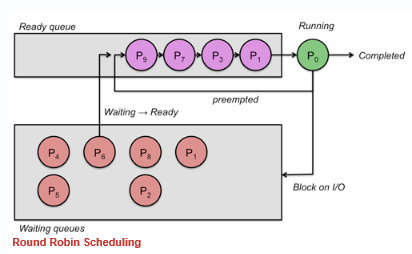
\includegraphics[width=.5\textwidth]{figuras/ilusrr}
	\caption{Simulação Round Robin} 
	\textbf{Fonte:} https://www.cs.rutgers.edu/ \cite{rutgers}
	\label{fig:figura-ilus2}
\end{figure}    

\subsection{Prioridades}  
 Cada processo recebe uma prioridade (número). O Round Robin assume que todos os processos são igualmente importantes. Isso geralmente não é o caso. Às vezes gostaríamos de ver processos longos (não interativos) com uso intensivo de CPU obterem uma prioridade menor que os processos interativos. Esses processos, por sua vez, devem ter uma prioridade menor que os trabalhos críticos para o sistema operacional.
Além disso, usuários diferentes podem ter status diferentes. Os processos de um administrador de sistema podem ser classificados acima dos de um aluno. 
Ignorando prioridades dinâmicas, o algoritmo de escalonamento de prioridades é direto: cada processo tem um número de prioridade atribuído a ele e o escalonador simplesmente escolhe o processo com a prioridade mais baixa. \cite{rutgers} 
\begin{itemize}
\item Vantagem: o escalonamento de prioridades fornece um bom mecanismo onde a importância relativa de cada processo pode ser definida com precisão.
\item Desvantagem: Se processos de alta prioridade consumirem muito tempo de CPU, processos de baixa prioridade podem passar fome e ser adiados indefinidamente, levando à inanição. 
\end{itemize} 
\subsubsection{Lidando com a fome}
Uma abordagem para o problema do adiamento indefinido é usar prioridades dinâmicas. Na expiração de cada quantum, o escalonador pode diminuir a prioridade do processo em execução atual (penalizando-o, portanto, por consumir tanto tempo da CPU). Eventualmente, sua prioridade ficará abaixo do próximo processo mais alto e esse processo poderá ser executado.
Outra abordagem é fazer com que o agendador acompanhe os processos de baixa prioridade que não têm a chance de executar e aumentar sua prioridade, de modo que, eventualmente, a prioridade seja alta o suficiente para que os processos sejam agendados para execução. Uma vez que é executado para o seu quantum, a prioridade pode ser trazida de volta ao nível baixo anterior.
Esse aumento periódico da prioridade de um processo para garantir que ele tenha uma chance de ser executado é chamado envelhecimento do processo. Uma maneira simples de implementar o envelhecimento é simplesmente aumentar a prioridade de cada processo e, em seguida, fazer com que eles sejam reajustados. \cite{tutorialspoint}  
  
\section{Códigos}   
\subsection{O arquivo main.py} 
\begin{lstlisting}
# -*- coding: utf-8 -*- 
import sys
import processo 
import escalonadores
import util

if len(sys.argv)  != 2: 
	printf("ERROR: Modo de uso: python main.py <arquivo de processos>")
	exit(1)
arq = open(sys.argv[1], 'r')
processos = util.formatarProcessos(arq,processo) 


# print processos

#fifo = escalonadores.FIFO(processos)
#fifo.executar()  

sjf = escalonadores.SJF(processos)  
sjf.executar()

#rr = escalonadores.RR(processos)   
#Passar o timeslice
#rr.executar(10)

#prioridades = escalonadores.PRIORIDADES(processos) 
#prioridades.executar()  
\end{lstlisting}  

\subsection{O arquivo processo.py}  
\begin{lstlisting}  
USUARIO = 0     # define usuario como 0
SISTEMA = 1     # define sistema como 1
class Processo(object):

tempos = {}
estado = None
eventos = []
tipo = None

def __init__(self, Id, prioridade, tempos, tam, estado, eventos):
	self.id = Id
	self.prioridade = prioridade
	self.tempos = tempos
	self.estado = estado
	self.eventos = eventos
	self.tamanho = tam
	self.tipo = USUARIO

def __str__(self):      #funcao de print de um objeto
	return "\n" + str(self.__dict__)

def __repr__(self):     #funcao de print de uma lista de objetos
	return str(self) + "\n"

def __getitem__(self, tup):     #recebe como parametro uma tupla que contem o nome do atributo e posicao; retorna o objeto
	nome, posi = tup
	return self.__getattribute__(nome)[posi]

class Sistema(Processo):

def __init__(self):
	self.tipo = SISTEMA

def exec_IO(self, processo, tempo_exec):
	if len(processo.eventos):
		print "Evento de IO do processo ID = {} executado no tempo: {}".format(processo.id, tempo_exec)
		processo.eventos.pop(0)
 
\end{lstlisting}  
 
\subsection{O arquivo util.py}  
\begin{lstlisting}
# -*- coding: utf-8 -*-
 
def formatarProcessos(arq,processo):    #formata uma lista de processos em uma lista de objetos
	processos = []
	texto = arq.readline()
	while texto:    #enquanto houver linhas para ler
		texto = texto.strip('\n')   #retira a quebra de linha
		content = texto.split(' ')  #passa para um vetor retirando o token " "
		idProcesso = content[0]
		tam = int(content[1])
		prioridade = content[2]
		tempo_chegada = content[3]
		eventos = []
	j = 0
	for i in range(4, len(content)):
		eventos.append(int(content[i]))
		if eventos[j] > tam-1:
			print "ERROR: Evento de IO fora do tempo do processo"
			exit(1)
		j+=1
	eventos.sort()
	processos.append(
		processo.Processo(
				idProcesso,
				prioridade,
				{"chegada" : int(tempo_chegada), "inicio" : None, "executado" : 0}, #None = tempo de inicio
				tam,
				"parado", # estado inicial
				eventos 
					)
	)
	texto = arq.readline()  #pula pra proxima linha
return processos
\end{lstlisting}
 
\subsection{O arquivo escalonadores.py} 
\begin{lstlisting}
# -*- coding: utf-8 -*-
import operator
import processo
class Escalonadores(object):

lista_espera = []   # lista de espera da execucao
ordem = []  #ordem de execucao
tempos = {"execucao" : 0, "espera" : 0}
lista_prontos = [] # lista de prontos para round robin   

def __init__(self, processos):
	self.processos = processos
def ordenar(self):
	pass
def executar(self, processo):
	pass

#class FIFO(Escalonadores):
#class SJF(Escalonadores): 
#class RR(Escalonadores): 
#class PRIORIDADES(Escalonadores):
\end{lstlisting} 
\subsubsection{Escalonador FIFO} 
\begin{lstlisting} 
class FIFO(Escalonadores):

def __init__(self, processos):
	super(FIFO,self).__init__(processos) #heranca da classe pai


def ordenar(self):
	self.ordem = sorted(self.processos, key = operator.itemgetter(("tempos","chegada"))) #ordena por ordem de chegada

self.ordem.append(processo.Sistema())       #coloca um processo do tipo sistema no final

def __str__(self):  #funcao de print de um objeto
	return "\n" + str(self.__dict__) 

def __repr__(self): #funcao de print de uma lista de objetos
	return str(self) + "\n" 


def esperar(self,processo): #espera o processo chegar
	while self.tempos["execucao"] < processo.tempos["chegada"]:
	self.tempos["execucao"] = self.tempos["execucao"] + 1 
	self.tempos["espera"] = self.tempos["espera"] + 1 

def executar_proc(self, processo): 
	while processo.tempos["executado"] < processo.tamanho:   #nao premptivo, nao pode ser parado ate que termine
	self.tempos["execucao"] = self.tempos["execucao"] + 1
	processo.tempos["executado"] = processo.tempos["executado"] + 1 

def bloqueiaProcIO(self, processo):
	self.lista_prontos.remove(processo)
	self.lista_espera.append(processo)

def executar(self): #funcao principal, executa os processos na ordem fifo
	self.ordenar()
	for i in range(len(self.ordem)):#para todos os processos
		if self.ordem[i].tipo == processo.USUARIO:  #se for processo de usuario
			self.esperar(self.ordem[i])
			self.lista_prontos.append(self.ordem[i])
			print("{} - {} # Processo {}".format(self.tempos["execucao"], (self.tempos["execucao"]+self.ordem[i].tamanho), self.ordem[i].id))
			self.executar_proc(self.ordem[i])
			if len(self.ordem[i].eventos):
				self.bloqueiaProcIO(self.ordem[i])
			else:
				self.lista_prontos.remove(self.ordem[i])
		else:# se for processo do sistema
			for j in range(len(self.lista_espera)):
				for k in range(len(self.lista_espera[j].eventos)):	
					self.ordem[i].exec_IO(self.lista_espera[j],self.tempos["execucao"]) 
					
self.lista_prontos = []

print("\nTempo total de execucao: {}ns".format(self.tempos["execucao"]))

print("Tempo total de espera: {}ns".format(self.tempos["espera"]))

print("Tempo medio de espera: {}ns".format((float(self.tempos["espera"]) / float(len(self.ordem)))))

\end{lstlisting}  
  
\section{Implementação} 
Para a implementação do simulador de gerenciamento de processos foi utilizada a linguagem Python. Também foram utilizados algumas noções sobre orientação a objeto como herança de classes. A ideia principal do código é a construção de processos completos para a realização de alguns tipos de escalonamento com a finalidade de diferenciar os métodos utilizados.   
\subsection{O arquivo main}
No arquivo principal é onde se recebe a entrada de processos existentes por meio de um arquivo de entrada, e logo em seguida escolhe-se o método de escalonamento utilizado para executar os processos.   
\subsection{O arquivo processos} 
Neste arquivo é criada a estrutura para armazenar as informações de um processo. Além do processo de usuário, também é criado um novo tipo de processo chamado "Sistema", ele é o responsável para realizar as entradas e saídas (I/O) quando terminar as execuções dos processos ou quando terminar uma rodada de execução no caso dos algoritmos preemptivos. Neste arquivo é definida a estrutura de um processo com todas suas variáveis e também funções para imprimir um processo ou uma tupla.
\subsection{O arquivo útil}  
O arquivo útil é extremamente necessário para a criação dos processos e  também seu preenchimento com os dados de entrada. É ele quem recebe o arquivo de entrada "\textit{input.txt}" e faz a transição dos dados para o programa utilizado de forma armazená-los de forma estruturada em um processo.
\subsection{O arquivo escalonadores} 
Neste arquivo a classe de escalonadores recebe os processos a serem escalonados e então são implementados dentro dele os métodos preemptivos e não preemptivos para escalonar os processos recebidos. Para auxiliar o trabalho do escalonador foi utilizado um vetor de processos chamado ordem, onde os processos serão ordenados por alguma característica como "tempo de chegada"(FIFO) ou "tamanho"(SJF). É fundamental também a utilização de uma lista de prontos e uma lista de espera para que o algoritmo contemple todos os estados possíveis de um processo, porém é responsabilidade do escalonador decidir por exemplo qual processo é despachado ou acordado em certo tempo. É fundamental que se armazene sempre o tempo total de execução e de espera.

\section{Gráficos e Diagramas}
Nesta seção são apresentados alguns resultados do trabalho como o diagrama de Gantt\cite{tanenbaum}, tempo total de execução e tempo médio de espera de cada algoritmo de escalonamento, com a finalidade de diferenciar as formas de se trabalhar com um escalonador e ainda mostrar algumas vantagens e desvantagens de cada método utilizado. Para poder comparar os resultados foi utilizada a seguinte entrada de dados (processos): 

\begin{figure}[!htb]
    \centering
    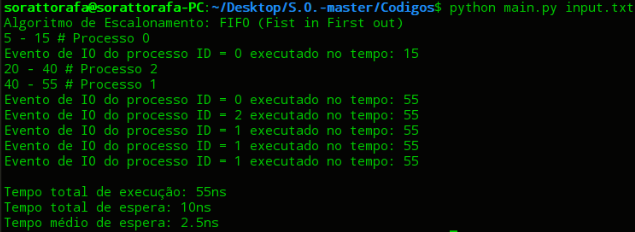
\includegraphics[width=.5\textwidth]{figuras/fifo}
    \caption{Escalonamento FIFO}
    \label{fig:figura-001}
\end{figure}   
 
\begin{figure}[!htb]
	\centering
	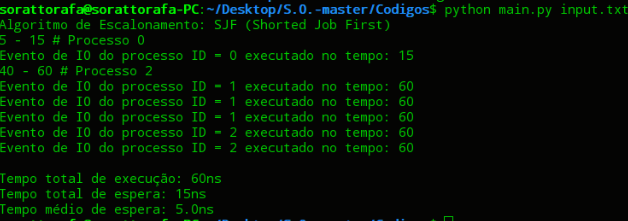
\includegraphics[width=.5\textwidth]{figuras/sjf}
	\caption{Escalonamento SJF}
	\label{fig:figura-002}
\end{figure}  


\begin{figure}[!htb]
	\centering
	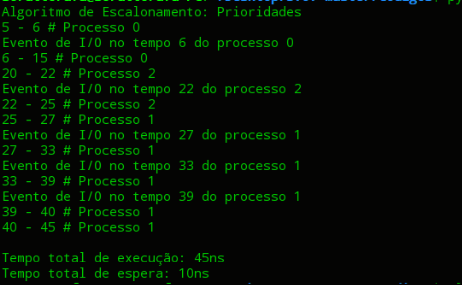
\includegraphics[width=.4\textwidth]{figuras/priori}
	\caption{Escalonamento Prioridades}
	\label{fig:figura-003}
\end{figure} 

\begin{figure}[!htb]
	\centering
	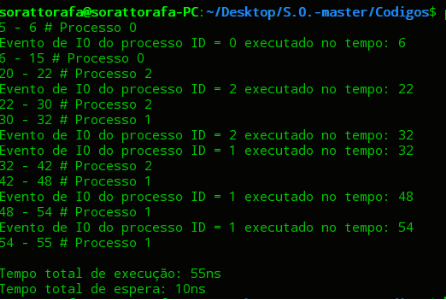
\includegraphics[width=.4\textwidth]{figuras/rr}
	\caption{Escalonamento Prioridades}
	\label{fig:figura-004}
\end{figure}



%A Figura~{\ref{fig:figura-003}}, apresenta um outro tipo de gráfico que pode ser utilizado, com já foi dito, qualquer tipo de gráfico pode ser utilizado para permitir ao leitor uma visualização de informações importantes.


%\begin{figure}[*H]
%    \centering
%    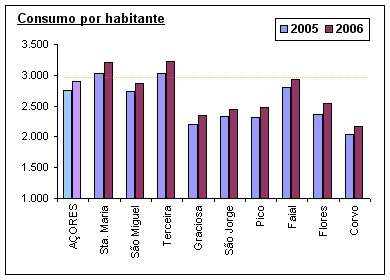
\includegraphics[width=.5\textwidth]{figuras/consumo-2.jpg}
%    \caption{Consumo de Energia 2}
%    \label{fig:figura-003}
%\end{figure}



\section{Blá Blá}

\section{Conclusão}


%------------------------------------------------------------------------- 
\nocite{ex1,ex2}
%\bibliography{bibliografia.bib}
\bibliographystyle{latex8}
\bibliography{bibliografia}

\end{document}
